\documentclass[letterpaper, 12pt]{article}
\usepackage[letterpaper, top=2.5cm, bottom=2.5cm, left=3cm, right=3cm]{geometry} %margenes
\usepackage[utf8]{inputenc} %manejo de caracteres especiales
\usepackage[spanish]{babel} %manejo de encabezados de inglés a español
\usepackage{fancyhdr} %formato de los encabezados de página
\usepackage{ragged2e} %alineado real justficado
\usepackage{graphicx} %manejo de imagenes
\usepackage{amsmath} %manejo de notación matemática
\usepackage{mathtools} %manejo de notación matemática
\usepackage{blindtext} %texto de relleno
\usepackage{cancel} %permite la simbolización de cancelación de terminos
\usepackage{enumitem}[shortlabels] %listas con letras
\usepackage{amssymb} %manejo de simbolog►1a matematica

\pagestyle{fancy}
\fancyhf{}
\rfoot{\thepage}

\begin{document}
\setcounter{page}{1}
\thispagestyle{fancy}
\lhead{\textbf{Tarea 3, U2}}
\rhead{\textbf{19/10/2020}}
\section*{Curvas planas, ecuaciones paramétricas y coordenadas polares}
\subsection*{Grafíca las siguientes ecuaciones: }
\[\begin{matrix}
    r_1=1-\cos\theta\\
    r_2=1+\cos\theta\\
    r_3=2+2\sin\theta\\
    r_4=2-2\sin\theta
\end{matrix}\]
\subsubsection*{Tabla de valores:}
\[\begin{matrix}
    \theta&0&\frac{\pi}{4}&\frac{\pi}{2}&\frac{3\pi}{4}&\pi&\frac{5\pi}{4}&\frac{3\pi}{2}&\frac{7\pi}{4}&2\pi\\
    r_1&0&0.29&1&1.71&2&1.71&1&0.29&0\\
    r_2&2&1.71&1&0.29&0&0.29&1&1.71&2\\
    r_3&2&3.41&4&3.41&2&0.59&0&0.59&2\\
    r_4&2&0.59&0&0.59&2&3.41&4&3.41&2
\end{matrix}\]
\subsubsection*{Gráficas:}
\[\begin{matrix}
    r_1=1-\cos\theta&\text{Azul}\\
    r_2=1+\cos\theta&\text{Rojo}
\end{matrix}\]
\begin{center}
    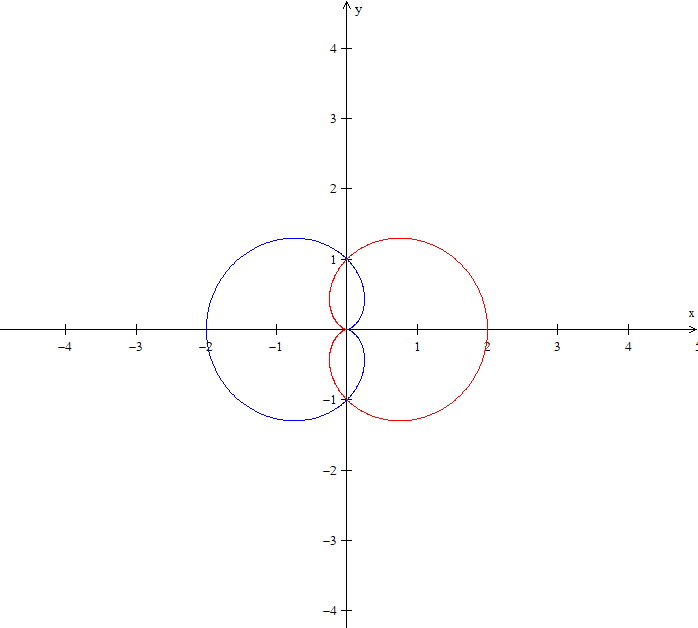
\includegraphics[width=11cm]{Capture.PNG}
\end{center}
\[\begin{matrix}
    r_3=2+2\sin\theta&\text{Azul}\\
    r_4=2-2\sin\theta&\text{Rojo}
\end{matrix}\]
\begin{center}
    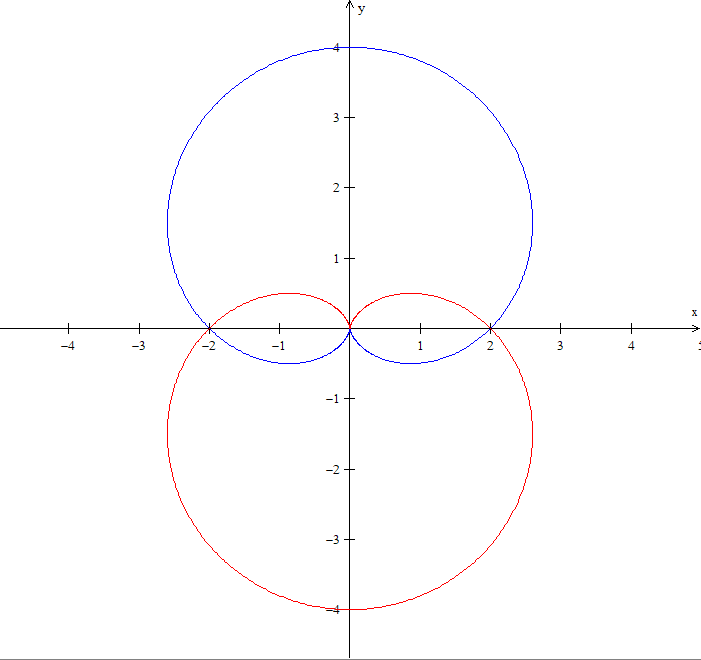
\includegraphics[width=11cm]{Capture2.PNG}
\end{center}
\end{document}